% This is file JFM2esam.tex
%   (based on JFMsampl.tex v1.3 for LaTeX2.09)
% Copyright (C) 1996, 1997, 2014 Cambridge University Press
\pdfoutput=1
\documentclass{jfm}
\usepackage{graphicx}
\usepackage{braket}
\usepackage{tabularx}
\usepackage{epstopdf, epsfig}
\usepackage[dvipsnames]{xcolor}
\usepackage{url}
\usepackage{multirow}
\usepackage{hhline}
\usepackage{comment}
\usepackage{longtable}
\usepackage{booktabs}
\usepackage{lipsum}  

\title{Titolo}
\shorttitle{Gruppo numero XX}
\shortauthor{Gruppo numero XX}

\author{
Primo componente\aff{1},
Secondo componente\aff{2},
Terzo componente\aff{3}
  % \corresp{\email{}}  
  }
\affiliation{
\aff{1}indirizzo email \& matricola del primo componente del gruppo
\aff{2}indirizzo email \& matricola del secondo componente del gruppo
\aff{3}indirizzo email \& matricola del terzo componente del gruppo
}

\begin{document}

\maketitle

% \begin{abstract}
% \end{abstract}

% \begin{keywords}
% \end{keywords}


\section{Esempio formule}
Esempio di citazione: \cite{drela89}

Esempio di equazione in linea: $c_L=2\pi(\alpha-\alpha_0)$.

Esempio di equazione in display:
\begin{equation}
    \alpha_{Th} = \frac 1 \pi \int_{-L/2}^{L/2} \frac{1}{\sqrt{\frac{L^2}{4}-s^2}}y'(s)\, {\rm d} s\,.
\end{equation}
\lipsum[1-3]

\section{Esempio figure}

Esempio di figura con riferimento: Figura~\ref{fig:nome_figura} (la posizione delle figure non è importante, l'importante è il riferimento nel testo!).
\begin{figure}
    \centering
    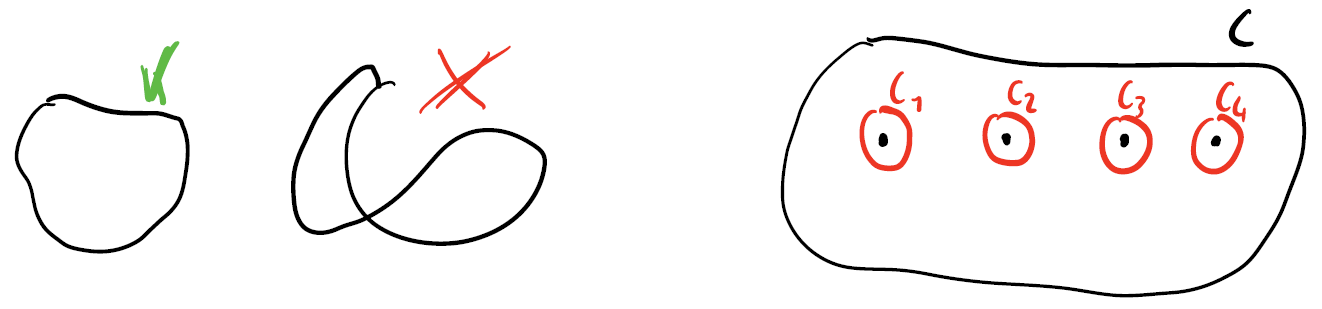
\includegraphics[width=0.5\textwidth]{figures/example.png}
    \caption{Figura di esampio.}
    \label{fig:nome_figura}
\end{figure}
\lipsum[4-6]

\section{Esempio tabella}

Esempio di tabella con riferimento: Tabella~\ref{tab:nome_tabella}.

\begin{table}
    \centering
    \begin{tabular}{c|c|c}
        profilo & $\alpha_{Th}$ \\
        NACA0006 & ?\\ 
        NACA0006 & ?\\
        NACA0006 & ?\\
    \end{tabular}
    \caption{Tabella di esampio.}
    \label{tab:nome_tabella}
\end{table}

\lipsum[7-9]

\bibliographystyle{jfm}
\bibliography{ms}
  \ifnum\value{page}>3
    \section*{{\color{red} NUMERO DI PAGINE MAGGIORE DI 3! LAUREA REVOCATA!}}
  \fi
\end{document}
